%! Author = Philipp Emmenegger
%! Date = 08/06/2021

\section{Software Architecture}
\textbf{Architecture} focuses on the big picture, the components, boundaries and interfaces.\\
\textbf{Design} addresses smaller challenges within these components\\
\textbf{Inputs for the architecture:}
\begin{itemize}
    \item Functional requirements
    \item Non-functional requirements
    \item Context
    \item Constraints
\end{itemize}

\subsection{Components}
\textbf{Separate by similarity}
\begin{itemize}
    \item Similar in functionality
    \item Similar in technological implementation
\end{itemize}
\textbf{Separate domain from technology}
\begin{itemize}
    \item Domain is stable and long living
    \item Technology is volatile and short living
\end{itemize}

\subsection{Layers vs. Tiers}
\textbf{Layers}
\begin{itemize}
    \item A way of organizing your code
    \item Logical separation by responsibility
\end{itemize}
\textbf{Tiers}
\begin{itemize}
    \item Define where layers are run and deployed
    \item Layers can beb deployed multiple times
\end{itemize}

\subsection{The big three}
\textbf{Adequacy (Angemessenheit)}
\begin{itemize}
    \item Design a system that fits: complexity, team, ...
    \item No Under / Over Engineering
    \item Do not reinvent the wheel
    \item Avoid the golden hammer
\end{itemize}
\textbf{Timeliness}
\begin{itemize}
    \item Eliminate risks early
    \item Decide at the last responsible moment
    \item Do not decite too late
    \item Use time to gather knowledge and experience
\end{itemize}
\textbf{Consistency}
\begin{itemize}
    \item Be consistent within your architecture
    \item Foster consistency using concepts
    \item Use existing concepts when appropriate
\end{itemize}

\subsection{Design}
\textbf{Top-Down}
\begin{itemize}
    \item Provides an overview
    \item Start with the big, work towards the small
    \item Perfect for documentation and communication
\end{itemize}
\textbf{Bottom-Up}
\begin{itemize}
    \item Addresses technical risks
    \item Solve a single problem, generalize afterwards
    \item Might lead to insufficient consistency
\end{itemize}

\subsection{Anti-Patterns}
\begin{itemize}
    \item Over Engineering
    \item Under Engineering
    \item Gold Hammer
    \item Reinvent the wheel
    \item Design in an ivory tower
    \item Design by power point
    \item Design by market
    \item Design for resume
\end{itemize}

\subsection{Documentation}
\begin{itemize}
    \item Correctness
    \item Maintainability
    \begin{itemize}
        \item use templates and standarts
    \end{itemize}
    \item Understandability
    \item Adequateness
\end{itemize}

\subsubsection{arc42 template}
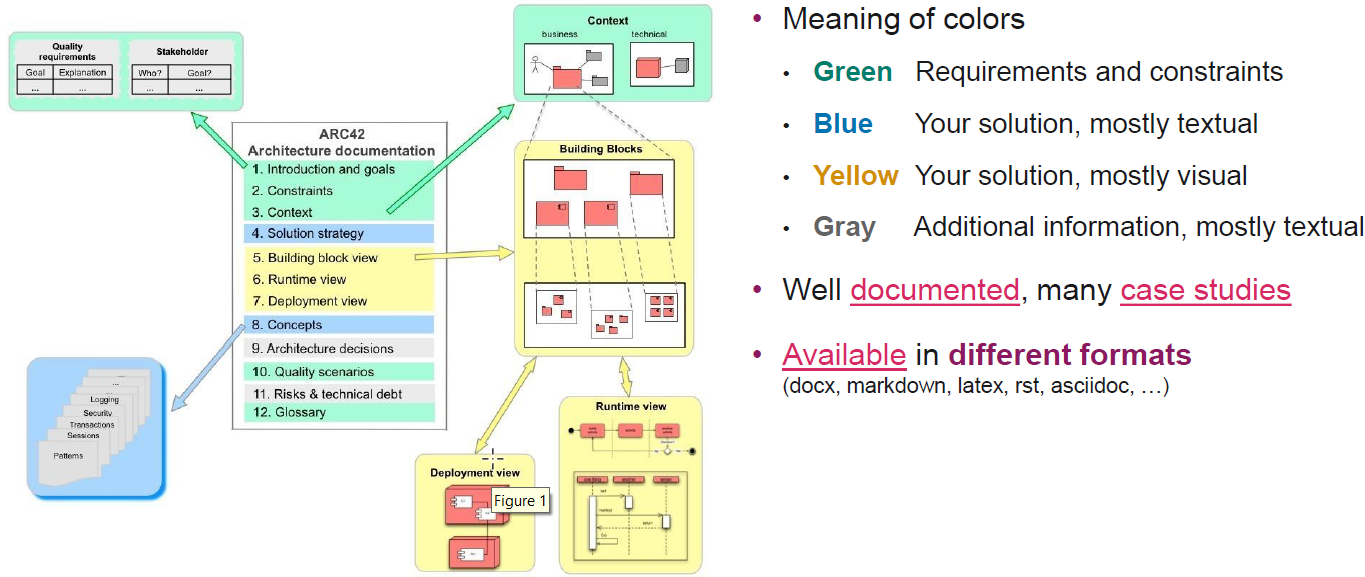
\includegraphics[width=\linewidth]{../img/arc42.png}

\subsection{Patterns}
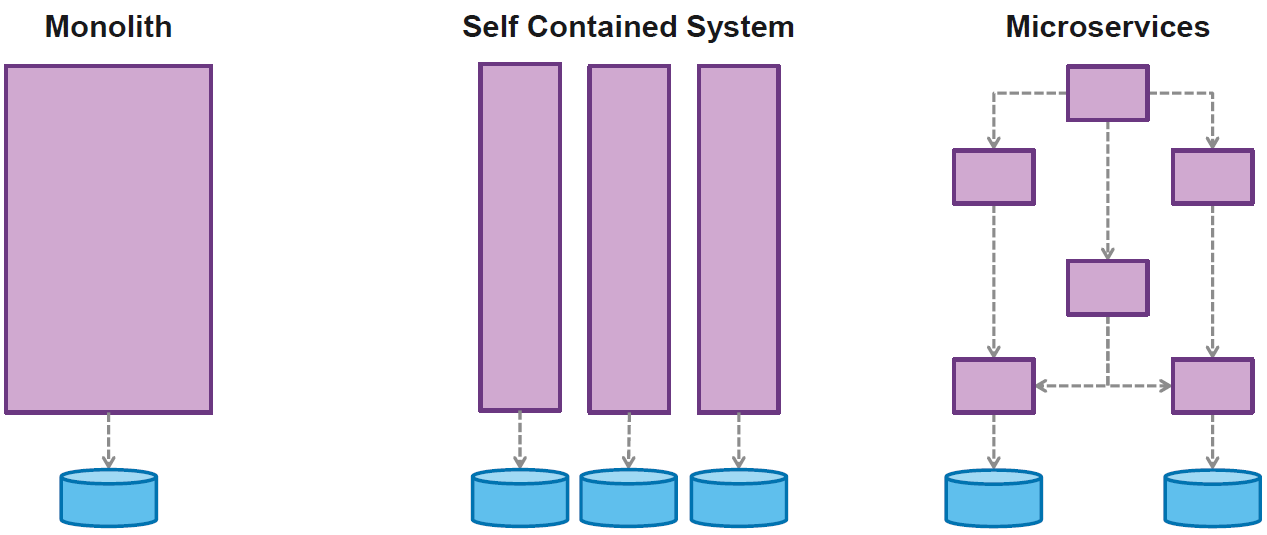
\includegraphics[width=\linewidth]{../img/architecture_patterns_1.png}
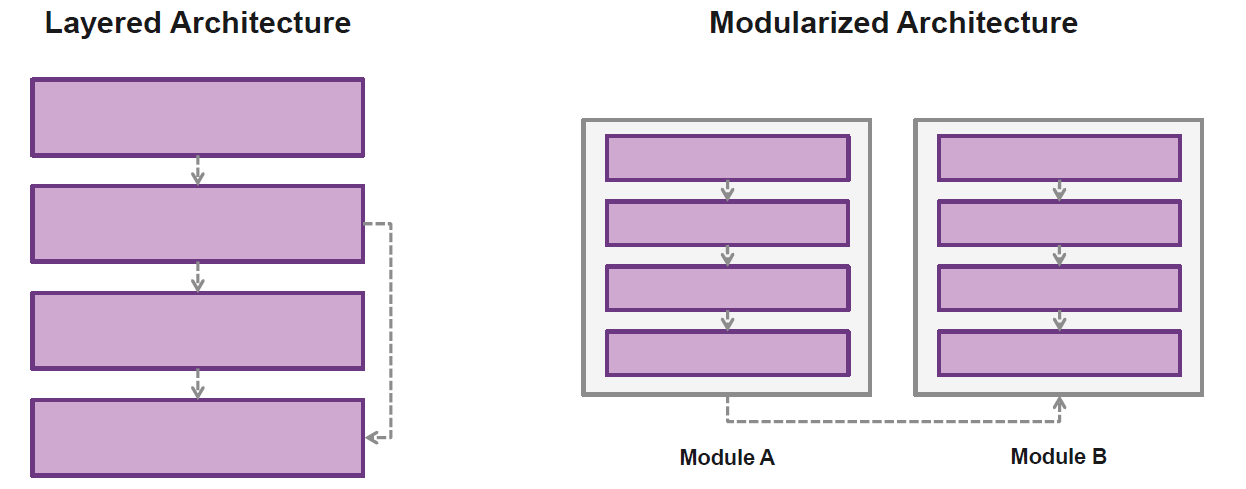
\includegraphics[width=\linewidth]{../img/architecture_patterns_2.png}
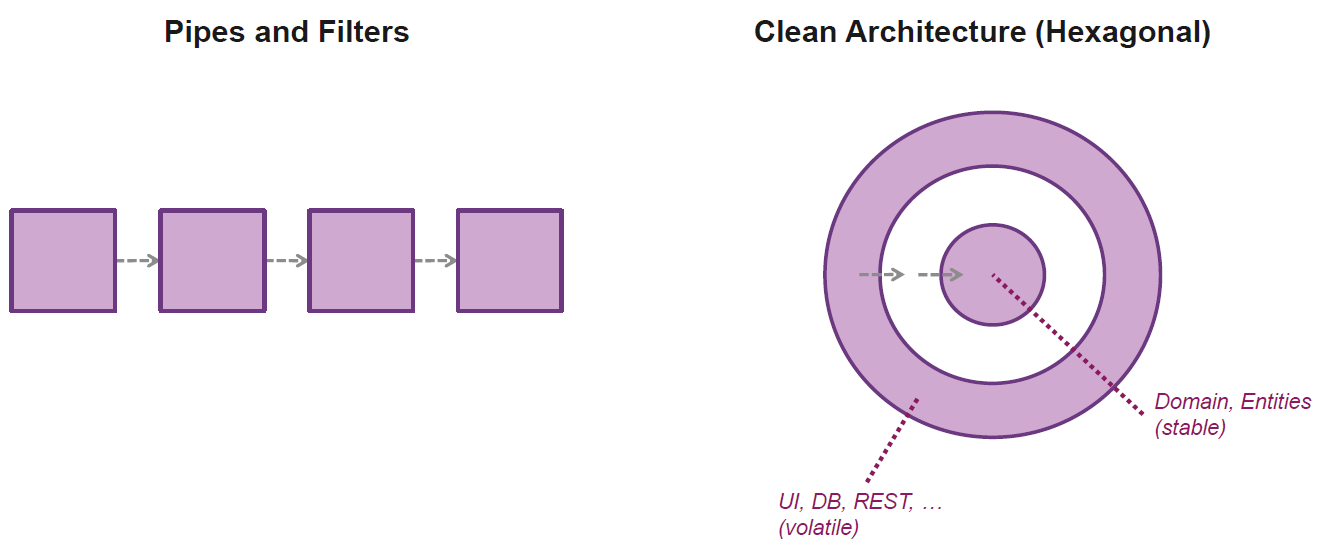
\includegraphics[width=\linewidth]{../img/architecture_patterns_3.png}











